\documentclass{beamer}
\usepackage{graphicx}
\begin{document}
\title{Array-Based Topological Mesh Representation
 Supporting General Modification}
\author{Dan Ibanez}

\frame{\titlepage}

\frame{\frametitle{Overview}
We present a mesh data structure with novel properties:
\begin{itemize}
\item composed of several large arrays
\item addition and removal are $O(1)$ operations
\item supports mixed element types
\item stores arbitrary associated data
\item uses 4x less memory than object-based versions
\end{itemize}
}

\frame{\frametitle{Basic Mesh Data Structure}
The simplest mesh data structure is an element to
node connectivity array.

Given an integer element id, returns the integer
node ids of that element.

Sufficient for element integration, element
stiffness matrix assembly, etc.

\vskip 20pt

\begin{center}
\includegraphics[width=0.4\textwidth]{ibanez_cse15-1.png}
\hspace{30pt}
\includegraphics[width=0.4\textwidth]{ibanez_cse15-2.png}
\end{center}
}

\frame{\frametitle{Adjacency Graph}
Element to node connectivity forms a bipartite graph
where all elements of the same topological type
have the same degree.

In the example, both elements are quadrilaterals.

\begin{center}
\includegraphics[width=0.6\textwidth]{ibanez_cse15-3.png}
\end{center}
}

\frame{\frametitle{Upward Adjacency}
The inverse of element-node connectivity, i.e.
which elements are adjacent to a node.

This is harder, because the degrees are not the same.

Object-based structures may store many small arrays.

\begin{center}
\includegraphics[width=0.6\textwidth]{ibanez_cse15-4.png}
\end{center}

Required during any kind of mesh modification, including
element load balancing.
}

\frame{\frametitle{Compact Upward Adjacency}
Assuming a mesh is static, the upward data
can be placed in one array.

Note that it is exactly the same size as the downward
array.

That is because {\emph each entry represents an adjacency
graph edge}, in both arrays.

\begin{center}
\includegraphics[width=0.6\textwidth]{ibanez_cse15-5.png}
\end{center}
}

\frame{\frametitle{Linked Upward Adjacency}
We can also rearrange the entries of the upward array
to match the ordering of the downward array, such
that the same graph edge has the same index.

\begin{center}
\includegraphics[width=0.6\textwidth]{ibanez_cse15-6.png}
\end{center}

Element id is now implicit by location, but
entries are non-contiguous and must be linked.
}

\frame{\frametitle{Upward Adjacency Arrays}
Since the element id can be derived from the entry's
position, we can use the entries to store list links
instead.
Another array for the nodes points to the head
of the list.

\begin{center}
\includegraphics[width=0.6\textwidth]{ibanez_cse15-7.png}
\end{center}

Array indices are used instead of pointers.
Upward adjacency can still be derived by traversing
these lists-in-arrays.
}

\frame{\frametitle{Upward Adjacency Rationale}

\begin{itemize}
\item
lists-in-array structure uses the same storage pattern
as contiguous arrays structure.
\item
Elements can be \emph{added} by growing the array
with new list nodes and linking them into the lists.
\item
Elements can be \emph{removed} by unlinking their list nodes
from the lists.
\item
However, unlinking from singly-linked list is $O($list size$)$,
which is $O($elements around vertex$)$. 
So, we assume that the latter is $O(1)$.
\end{itemize}

\begin{center}
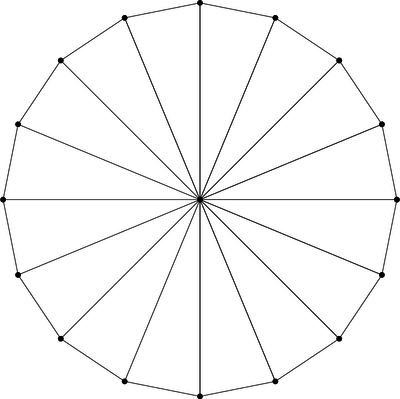
\includegraphics[width=0.3\textwidth]{fan.png}
\end{center}
}

\frame{\frametitle{Mesh Modification}
\begin{itemize}
\item
All mesh modifications are implemented as element
addition and removal.

\item
We have arrays of size $CN$ where $N$ is the
number of entities of one type,
and each $C$ contiguous entries
correspond to the same entity.

\item
We need general array modification algorithms
for adding and removing entries
(or contiguous $C$ entries).

\item
Finally, we control where addition happens, users
just want storage for a new entity.
\end{itemize}
}

\frame{\frametitle{Array Addition}
\begin{itemize}
\item
Common solution is geometric growth with additions to the end.
For example, the C++ std::vector uses this algorithm.
\item
Array has allocated capacity $(c)$ and used size.
When addition is requested and used size equals capacity,
reallocate to capacity $\alpha c$, $\alpha > 1$.
We use $\frac32(c+1)$.
\item
Result is amortized $O(1)$ insertion at the end.
\item
{\bf C}'s \texttt{realloc()} can be more efficient due
to virtual memory page mapping...
\end{itemize}
\begin{center}
\includegraphics[width=0.4\textwidth]{ibanez_cse15-9.png}
\end{center}
}

\frame{\frametitle{Array Removal}
\begin{itemize}
\item
Removal can happen anywhere, leaves a hole.
\item
Trying to fill the hole requires moving another
entry or entries
\item
But changing indices is bad for users, they
need unique consistent identifiers
\item
So, keep the holes and track them
\end{itemize}
}

\frame{\frametitle{Free List}
\begin{itemize}
\item
One array per entity type, tracks holes in other arrays
\item
Holes are linked together in one ``free list".
\item
On removal, new hole is linked to front of list.
\item
On addition, check for holes and, if any, unlink
the first hole from the list and fill it.
\item
Non-holes receive a ``Live" value (-2) to distinguish
from valid linked list values $[-1,\infty)$.
\end{itemize}

\begin{center}
\includegraphics[width=0.6\textwidth]{ibanez_cse15-8.png}
\end{center}
}

\frame{\frametitle{Array Modification Algorithm}
On removal, link new hole into free list.

On addition:
\begin{enumerate}
\item
If there are holes, unlink the first hole
and return its index
\item
If used size equals capacity, reallocate for
bigger capacity
\item
Increment used size, return last index
\end{enumerate}

\vspace{20pt}

\includegraphics[width=0.8\textwidth]{flex.png}

}

\frame{\frametitle{Element-Vertex Structure}

A reduced mesh representation with only elements
and vertices would use the following set of arrays:

\begin{itemize}
\item Vertex free list array
\item Element free list array
\item Element to vertex array
\item Vertex to element lists-in-arrays
\item Simulation field arrays, indexed by vertex id
\end{itemize}

\begin{center}
\end{center}
}

\frame{\frametitle{Full Topological Representation}
For flexible adaptive meshes, as well as for simulations
with high-order field nodes, it is useful to represent
multiple dimensions of entities. 
The presence of edges and faces greatly simplifies
mesh adaptation code.
\begin{columns}[T]
\begin{column}{0.4\textwidth}
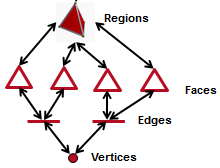
\includegraphics[width=\textwidth]{full.png}
\end{column}
\begin{column}{0.6\textwidth}
\includegraphics[width=\textwidth]{mia.png}
\end{column}
\end{columns}
To do this, create upward/downward relation arrays
for each pair of entity types.
Above is an edges-to-triangles example.
}

\frame{\frametitle{Full Topological Structure}
\begin{itemize}
\item free list array per dimension (4)
\item downward array per dimension (3)
\item upward arrays per dimension (6)
\item additional fields, indexed by entity id
\end{itemize}
Operations
\begin{itemize}
\item Add entity and set one-level up/down adjacencies
\item Remove entity
\item Query one-level upward adjacency
\item Query one-level downward adjacency
\item Iterate (increment, skip holes)
\end{itemize}
}

\frame{\frametitle{Mixed Meshes}
\begin{itemize}
\item Multiple topological types per dimension
\item Each per-dimension array is split into
per-type arrays
\item 2D array indices are encoded as $e = iT + t$,
where $T$ is the number of types, $t$ is entity type,
$i$ is index in array.
\item this applies to downward arrays, upward list arrays,
and additional field arrays.
\end{itemize}

\begin{center}
\includegraphics[width=0.5\textwidth]{ibanez_cse15-10.png}
\end{center}
}

\frame{\frametitle{Memory Analysis}
\begin{itemize}
\item consider full one-level tetrahedral mesh
\item static pointers =
$(4+4)n_{tet} + (1+3+3)n_{tri} + (1+2+2)n_{edg} + (1)n_{vtx}$
\item with free list =
$(1+4+4)n_{tet} + (1+1+3+3)n_{tri} + (1+1+2+2)n_{edg} + (1+1)n_{vtx}$
\item estimated ratios
\[n_{vtx} = n_{edg}/7 = n_{tri}/12 = n_{tet}/6\]
\item with free list, 194 pointers per vertex, 33 pointers per element
\item using 32-bit index ``pointers", 130 bytes per element
\item with non-topological data added, uses 250 bytes
per element
\item 4X less than before (from 1KB down to 250B per element)
\end{itemize}
}

\frame{\frametitle{Memory Measurement}
This array structure is implemented as a sub-component
of the PUMI tools, storing a full representation:

\vspace{10pt}
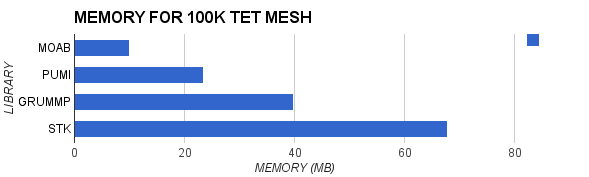
\includegraphics[width=\textwidth]{memuse.png}
\vspace{10pt}

Comparisons where made to MOAB from
Argonne National Labs, STK from Sandia National Labs,
and GRUMMP from UBC.

Note that MOAB is not representing edges or faces
and is not designed to add/remove entities individually.

}

\end{document}
